\subsection{Missing Energy}
The missing transverse energy vector is calculated offline as the
negative of the vector sum of transverse momenta of all PF candidates
identified in the event. The magnitude of this vector is referred to
as $E_{T}^{miss}$. To recover from the 
performance degradation of the missing transverse energy due to pile-up
interactions, we also consider the $H_{T}^{miss}$ variable, computed in
the same way as the $E_{T}^{miss}$, but using only the
selected jets and leptons (the lepton selection will be described in
the following paragraphs).  The $H_{T}^{miss}$ variable has worse
resolution than $E_{T}^{miss}$ but is more robust as it does
not rely on the soft part of the event.  In this analysis the event
selection makes use of a linear discriminator based on the two
variables, $E_{T}^{miss}LD$, exploiting the fact that $E_{T}^{miss}$
and $H_{T}^{miss}$ are less correlated in events with instrumental
missing energy with respect to events with real missing energy.
The $E_{T}^{miss}LD$ is defined as
\begin{equation}
 E_{T}^{miss}LD= E_{T}^{miss}*0.00397 + H_{T}^{miss}*0.00265
\label{eq:reconstruction_isolation}
\end{equation}
and the working point used is
$E_{T}^{miss}LD>0.2$, as in HIG-15-008.
%%%Fig.\,\ref{fig:met} shows the correlation
%%%between $H_{T}^{miss}$ and $E_{T}^{miss}$ in signal events and
%%%DY+jets events and the comparison between the performances of the two
%%%variables and the linear discriminator.


%%%\begin{figure}[htb]
%%%\centering
%%%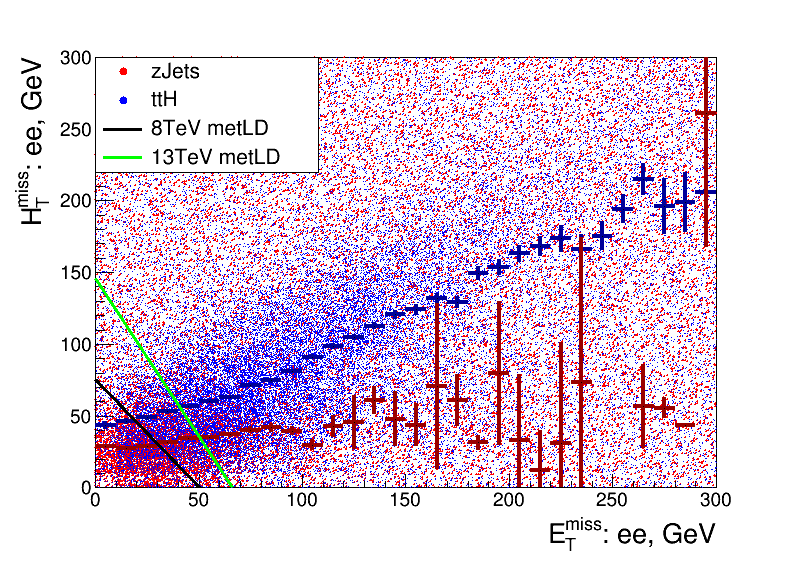
\includegraphics[width=0.50\linewidth]{plots_met/2Dplot_metld_ee.png} 
%%%\caption{The figure shows the correlation between the
%%%$H_{T}^{miss}$ and $E_{T}^{miss}$ variables in signal events (blue) and
%%%DY+jets events (red). This analysis uses the 
%%%\emph{8 TeV met LD} cut.} 
%%%\label{fig:met}
%%%\end{figure}
